

\tikzset{every picture/.style={line width=0.75pt}} %set default line width to 0.75pt        

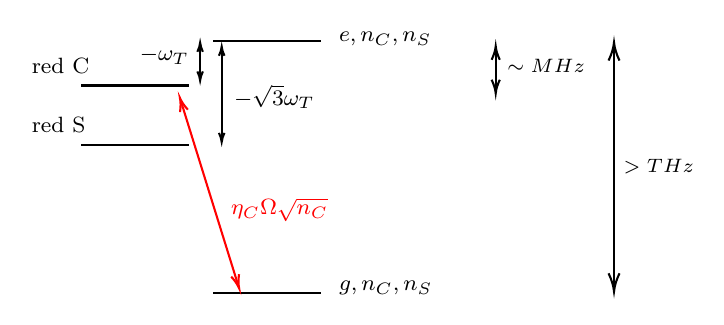
\begin{tikzpicture}[x=0.75pt,y=0.75pt,yscale=-1,xscale=1]
%uncomment if require: \path (0,146); %set diagram left start at 0, and has height of 146

%Straight Lines [id:da8993089849930328] 
\draw    (30.38,59.59) -- (82.31,59.59) ;
%Straight Lines [id:da29699103187525655] 
\draw    (30.38,30.75) -- (82.31,30.75) ;
%Straight Lines [id:da9565575071502495] 
\draw    (93.89,130.93) -- (145.83,130.93) ;
%Straight Lines [id:da38723274535804597] 
\draw    (93.89,9.5) -- (145.83,9.5) ;
%Straight Lines [id:da7230830907382644] 
\draw    (87.59,12.14) -- (87.59,26.36) ;
\draw [shift={(87.59,28.36)}, rotate = 270] [color={rgb, 255:red, 0; green, 0; blue, 0 }  ][line width=0.75]    (4.37,-1.32) .. controls (2.78,-0.56) and (1.32,-0.12) .. (0,0) .. controls (1.32,0.12) and (2.78,0.56) .. (4.37,1.32)   ;
\draw [shift={(87.59,10.14)}, rotate = 90] [color={rgb, 255:red, 0; green, 0; blue, 0 }  ][line width=0.75]    (4.37,-1.32) .. controls (2.78,-0.56) and (1.32,-0.12) .. (0,0) .. controls (1.32,0.12) and (2.78,0.56) .. (4.37,1.32)   ;
%Straight Lines [id:da7613574342882506] 
\draw    (97.98,14.06) -- (97.98,55.96) ;
\draw [shift={(97.98,57.96)}, rotate = 270] [color={rgb, 255:red, 0; green, 0; blue, 0 }  ][line width=0.75]    (4.37,-1.32) .. controls (2.78,-0.56) and (1.32,-0.12) .. (0,0) .. controls (1.32,0.12) and (2.78,0.56) .. (4.37,1.32)   ;
\draw [shift={(97.98,12.06)}, rotate = 90] [color={rgb, 255:red, 0; green, 0; blue, 0 }  ][line width=0.75]    (4.37,-1.32) .. controls (2.78,-0.56) and (1.32,-0.12) .. (0,0) .. controls (1.32,0.12) and (2.78,0.56) .. (4.37,1.32)   ;
%Straight Lines [id:da17453665512381966] 
\draw [color={rgb, 255:red, 255; green, 0; blue, 0 }  ,draw opacity=1 ]   (78.43,38.62) -- (105.81,126.62) ;
\draw [shift={(106.4,128.53)}, rotate = 252.72] [color={rgb, 255:red, 255; green, 0; blue, 0 }  ,draw opacity=1 ][line width=0.75]    (6.56,-1.97) .. controls (4.17,-0.84) and (1.99,-0.18) .. (0,0) .. controls (1.99,0.18) and (4.17,0.84) .. (6.56,1.97)   ;
\draw [shift={(77.84,36.71)}, rotate = 72.72] [color={rgb, 255:red, 255; green, 0; blue, 0 }  ,draw opacity=1 ][line width=0.75]    (6.56,-1.97) .. controls (4.17,-0.84) and (1.99,-0.18) .. (0,0) .. controls (1.99,0.18) and (4.17,0.84) .. (6.56,1.97)   ;
%Straight Lines [id:da35411700829971027] 
\draw    (287,12) -- (287,128) ;
\draw [shift={(287,130)}, rotate = 270] [color={rgb, 255:red, 0; green, 0; blue, 0 }  ][line width=0.75]    (8.74,-2.63) .. controls (5.56,-1.12) and (2.65,-0.24) .. (0,0) .. controls (2.65,0.24) and (5.56,1.12) .. (8.74,2.63)   ;
\draw [shift={(287,10)}, rotate = 90] [color={rgb, 255:red, 0; green, 0; blue, 0 }  ][line width=0.75]    (8.74,-2.63) .. controls (5.56,-1.12) and (2.65,-0.24) .. (0,0) .. controls (2.65,0.24) and (5.56,1.12) .. (8.74,2.63)   ;
%Straight Lines [id:da3640218170366485] 
\draw    (230,13.8) -- (230,32.55) ;
\draw [shift={(230,34.55)}, rotate = 270] [color={rgb, 255:red, 0; green, 0; blue, 0 }  ][line width=0.75]    (6.56,-1.97) .. controls (4.17,-0.84) and (1.99,-0.18) .. (0,0) .. controls (1.99,0.18) and (4.17,0.84) .. (6.56,1.97)   ;
\draw [shift={(230,11.8)}, rotate = 90] [color={rgb, 255:red, 0; green, 0; blue, 0 }  ][line width=0.75]    (6.56,-1.97) .. controls (4.17,-0.84) and (1.99,-0.18) .. (0,0) .. controls (1.99,0.18) and (4.17,0.84) .. (6.56,1.97)   ;

% Text Node
\draw (153,123.4) node [anchor=north west][inner sep=0.75pt]  [font=\footnotesize]  {$\ket{g,n_{C} ,n_{S}}$};
% Text Node
\draw (153,3.4) node [anchor=north west][inner sep=0.75pt]  [font=\footnotesize]  {$\ket{e,n_{C} ,n_{S}}$};
% Text Node
\draw (57,10.9) node [anchor=north west][inner sep=0.75pt]  [font=\footnotesize]  {$-\omega _{T}$};
% Text Node
\draw (102.5,28.9) node [anchor=north west][inner sep=0.75pt]  [font=\footnotesize]  {$-\sqrt{3} \omega _{T}$};
% Text Node
\draw (5,16) node [anchor=north west][inner sep=0.75pt]  [font=\footnotesize] [align=left] {red C};
% Text Node
\draw (5,44.5) node [anchor=north west][inner sep=0.75pt]  [font=\footnotesize] [align=left] {red S};
% Text Node
\draw (290,64.63) node [anchor=north west][inner sep=0.75pt]  [font=\scriptsize]  {$ >THz$};
% Text Node
\draw (234,16.43) node [anchor=north west][inner sep=0.75pt]  [font=\scriptsize]  {$\sim MHz$};
% Text Node
\draw (101,83.63) node [anchor=north west][inner sep=0.75pt]  [font=\footnotesize,color={rgb, 255:red, 255; green, 0; blue, 0 }  ,opacity=1 ]  {$\eta_C \Omega \sqrt{n_{C}}$};


\end{tikzpicture}
